% Options for packages loaded elsewhere
\PassOptionsToPackage{unicode}{hyperref}
\PassOptionsToPackage{hyphens}{url}
%
\documentclass[
  man]{apa6}
\usepackage{amsmath,amssymb}
\usepackage{lmodern}
\usepackage{iftex}
\ifPDFTeX
  \usepackage[T1]{fontenc}
  \usepackage[utf8]{inputenc}
  \usepackage{textcomp} % provide euro and other symbols
\else % if luatex or xetex
  \usepackage{unicode-math}
  \defaultfontfeatures{Scale=MatchLowercase}
  \defaultfontfeatures[\rmfamily]{Ligatures=TeX,Scale=1}
\fi
% Use upquote if available, for straight quotes in verbatim environments
\IfFileExists{upquote.sty}{\usepackage{upquote}}{}
\IfFileExists{microtype.sty}{% use microtype if available
  \usepackage[]{microtype}
  \UseMicrotypeSet[protrusion]{basicmath} % disable protrusion for tt fonts
}{}
\makeatletter
\@ifundefined{KOMAClassName}{% if non-KOMA class
  \IfFileExists{parskip.sty}{%
    \usepackage{parskip}
  }{% else
    \setlength{\parindent}{0pt}
    \setlength{\parskip}{6pt plus 2pt minus 1pt}}
}{% if KOMA class
  \KOMAoptions{parskip=half}}
\makeatother
\usepackage{xcolor}
\IfFileExists{xurl.sty}{\usepackage{xurl}}{} % add URL line breaks if available
\IfFileExists{bookmark.sty}{\usepackage{bookmark}}{\usepackage{hyperref}}
\hypersetup{
  pdftitle={A Conceptual Replication of Rothman (2011): L3 Syntactic Transfer Selectivity and Typological Determinacy: The Typological Primacy Model},
  pdfauthor={Kyle Parrish1},
  pdflang={en-EN},
  pdfkeywords={keywords},
  hidelinks,
  pdfcreator={LaTeX via pandoc}}
\urlstyle{same} % disable monospaced font for URLs
\usepackage{longtable,booktabs,array}
\usepackage{calc} % for calculating minipage widths
% Correct order of tables after \paragraph or \subparagraph
\usepackage{etoolbox}
\makeatletter
\patchcmd\longtable{\par}{\if@noskipsec\mbox{}\fi\par}{}{}
\makeatother
% Allow footnotes in longtable head/foot
\IfFileExists{footnotehyper.sty}{\usepackage{footnotehyper}}{\usepackage{footnote}}
\makesavenoteenv{longtable}
\usepackage{graphicx}
\makeatletter
\def\maxwidth{\ifdim\Gin@nat@width>\linewidth\linewidth\else\Gin@nat@width\fi}
\def\maxheight{\ifdim\Gin@nat@height>\textheight\textheight\else\Gin@nat@height\fi}
\makeatother
% Scale images if necessary, so that they will not overflow the page
% margins by default, and it is still possible to overwrite the defaults
% using explicit options in \includegraphics[width, height, ...]{}
\setkeys{Gin}{width=\maxwidth,height=\maxheight,keepaspectratio}
% Set default figure placement to htbp
\makeatletter
\def\fps@figure{htbp}
\makeatother
\setlength{\emergencystretch}{3em} % prevent overfull lines
\providecommand{\tightlist}{%
  \setlength{\itemsep}{0pt}\setlength{\parskip}{0pt}}
\setcounter{secnumdepth}{-\maxdimen} % remove section numbering
% Make \paragraph and \subparagraph free-standing
\ifx\paragraph\undefined\else
  \let\oldparagraph\paragraph
  \renewcommand{\paragraph}[1]{\oldparagraph{#1}\mbox{}}
\fi
\ifx\subparagraph\undefined\else
  \let\oldsubparagraph\subparagraph
  \renewcommand{\subparagraph}[1]{\oldsubparagraph{#1}\mbox{}}
\fi
\newlength{\cslhangindent}
\setlength{\cslhangindent}{1.5em}
\newlength{\csllabelwidth}
\setlength{\csllabelwidth}{3em}
\newlength{\cslentryspacingunit} % times entry-spacing
\setlength{\cslentryspacingunit}{\parskip}
\newenvironment{CSLReferences}[2] % #1 hanging-ident, #2 entry spacing
 {% don't indent paragraphs
  \setlength{\parindent}{0pt}
  % turn on hanging indent if param 1 is 1
  \ifodd #1
  \let\oldpar\par
  \def\par{\hangindent=\cslhangindent\oldpar}
  \fi
  % set entry spacing
  \setlength{\parskip}{#2\cslentryspacingunit}
 }%
 {}
\usepackage{calc}
\newcommand{\CSLBlock}[1]{#1\hfill\break}
\newcommand{\CSLLeftMargin}[1]{\parbox[t]{\csllabelwidth}{#1}}
\newcommand{\CSLRightInline}[1]{\parbox[t]{\linewidth - \csllabelwidth}{#1}\break}
\newcommand{\CSLIndent}[1]{\hspace{\cslhangindent}#1}
\ifLuaTeX
\usepackage[bidi=basic]{babel}
\else
\usepackage[bidi=default]{babel}
\fi
\babelprovide[main,import]{english}
% get rid of language-specific shorthands (see #6817):
\let\LanguageShortHands\languageshorthands
\def\languageshorthands#1{}
% Manuscript styling
\usepackage{upgreek}
\captionsetup{font=singlespacing,justification=justified}

% Table formatting
\usepackage{longtable}
\usepackage{lscape}
% \usepackage[counterclockwise]{rotating}   % Landscape page setup for large tables
\usepackage{multirow}		% Table styling
\usepackage{tabularx}		% Control Column width
\usepackage[flushleft]{threeparttable}	% Allows for three part tables with a specified notes section
\usepackage{threeparttablex}            % Lets threeparttable work with longtable

% Create new environments so endfloat can handle them
% \newenvironment{ltable}
%   {\begin{landscape}\centering\begin{threeparttable}}
%   {\end{threeparttable}\end{landscape}}
\newenvironment{lltable}{\begin{landscape}\centering\begin{ThreePartTable}}{\end{ThreePartTable}\end{landscape}}

% Enables adjusting longtable caption width to table width
% Solution found at http://golatex.de/longtable-mit-caption-so-breit-wie-die-tabelle-t15767.html
\makeatletter
\newcommand\LastLTentrywidth{1em}
\newlength\longtablewidth
\setlength{\longtablewidth}{1in}
\newcommand{\getlongtablewidth}{\begingroup \ifcsname LT@\roman{LT@tables}\endcsname \global\longtablewidth=0pt \renewcommand{\LT@entry}[2]{\global\advance\longtablewidth by ##2\relax\gdef\LastLTentrywidth{##2}}\@nameuse{LT@\roman{LT@tables}} \fi \endgroup}

% \setlength{\parindent}{0.5in}
% \setlength{\parskip}{0pt plus 0pt minus 0pt}

% Overwrite redefinition of paragraph and subparagraph by the default LaTeX template
% See https://github.com/crsh/papaja/issues/292
\makeatletter
\renewcommand{\paragraph}{\@startsection{paragraph}{4}{\parindent}%
  {0\baselineskip \@plus 0.2ex \@minus 0.2ex}%
  {-1em}%
  {\normalfont\normalsize\bfseries\itshape\typesectitle}}

\renewcommand{\subparagraph}[1]{\@startsection{subparagraph}{5}{1em}%
  {0\baselineskip \@plus 0.2ex \@minus 0.2ex}%
  {-\z@\relax}%
  {\normalfont\normalsize\itshape\hspace{\parindent}{#1}\textit{\addperi}}{\relax}}
\makeatother

% \usepackage{etoolbox}
\makeatletter
\patchcmd{\HyOrg@maketitle}
  {\section{\normalfont\normalsize\abstractname}}
  {\section*{\normalfont\normalsize\abstractname}}
  {}{\typeout{Failed to patch abstract.}}
\patchcmd{\HyOrg@maketitle}
  {\section{\protect\normalfont{\@title}}}
  {\section*{\protect\normalfont{\@title}}}
  {}{\typeout{Failed to patch title.}}
\makeatother

\usepackage{xpatch}
\makeatletter
\xapptocmd\appendix
  {\xapptocmd\section
    {\addcontentsline{toc}{section}{\appendixname\ifoneappendix\else~\theappendix\fi\\: #1}}
    {}{\InnerPatchFailed}%
  }
{}{\PatchFailed}
\keywords{keywords\newline\indent Word count: X}
\DeclareDelayedFloatFlavor{ThreePartTable}{table}
\DeclareDelayedFloatFlavor{lltable}{table}
\DeclareDelayedFloatFlavor*{longtable}{table}
\makeatletter
\renewcommand{\efloat@iwrite}[1]{\immediate\expandafter\protected@write\csname efloat@post#1\endcsname{}}
\makeatother
\usepackage{lineno}

\linenumbers
\usepackage{csquotes}
\ifLuaTeX
  \usepackage{selnolig}  % disable illegal ligatures
\fi

\title{A Conceptual Replication of Rothman (2011): L3 Syntactic Transfer Selectivity and Typological Determinacy: The Typological Primacy Model}
\author{Kyle Parrish\textsuperscript{1}}
\date{}


\shorttitle{Rothman (2011) Replication}

\authornote{

Add complete departmental affiliations for each author here. Each new line herein must be indented, like this line.

Enter author note here.

Correspondence concerning this article should be addressed to Kyle Parrish, 15 Seminary Place, New Brunswick, NJ. E-mail: \href{mailto:kyle.parrish@rutgers.edu}{\nolinkurl{kyle.parrish@rutgers.edu}}

}

\affiliation{\vspace{0.5cm}\textsuperscript{1} Rutgers University}

\abstract{%
This study partially replicated Rothman (2011), who found no effects between two L3 groups in thier perception and production of determiner phrase syntax.
The current study included a large sample (n = 211) of L3 learners of Portuguese.
These learners were divided into two groups in a mirror-image design (96 L1 English-L2 Spanish , 115 L1 Spanish-L2 English).
The original materials, a collocation task to measure production and a semantic interpretation task to measure perception, were recreated.
Like the original study, there was not a main effect for group in any of the two-way ANOVAs.
However, out of four total post-hoc tests of equivalence, only two were significant when the equivalence bounds were set at a small effect size.
Ultimately, it is argued that determining the smallest effect size of interest and subsequent equivalence testing are necessary to answer key questions in the field of L3 acquistion.
}



\begin{document}
\maketitle

\hypertarget{introduction}{%
\section{Introduction}\label{introduction}}

Since the early 2000s, the field of third language acquisition has emerged, with, in part, the goal of demonstrating that second language (L2) and third language (L3) learning are distinct processes.
One clear difference between L2 and L3 learners is their number of previously learned languages.
While L2 learners only speak one additional language, L3 learners, by definition, speak two languages in addition to the one that they are learning.
In L2 learning, the differences between a learner's native language and their L2 has been shown to predict its difficulty in learning.
This is the case because of cross-linguistic influence/transfer, where native language categories have been found to constitute the initial state of the new language (Schwartz \& Sprouse, 1996).
In the case of L3 learning, however, the initial state of learning is less clear.
Evidence indicates that L3 learners may be influenced in some cases by their L1 (Hermas, 2010) but by either their L2 (Bardel \& Falk, 2007), or by both languages in other cases (Westergaard, Mitrofanova, Mykhaylyk, \& Rodina, 2017).
As a result, several models of L3 acquisition have emerged with conflicting predictions related to previous language influence during the process of acquisition.

The present study was a conceptual replication of Rothman (2011).
In Rothman (2011), an influential model in L3 acquisition was proposed following two experiments: the Typological Primacy Model (the TPM).
The model predicts that the more one of two possible source language (between the L1 and L2) will wholly transfer to the L3 based on the parsing of hierarchical cues in L3 input (Rothman, 2015).
In the original study, the determiner phrase syntax of two groups of L3 learners were tested using a semantic interpretation task and a context-based Collocation Task.
Specifically, the study examined how pre and postnominal adjectives impacted noun meaning, which is present in Romance languages, but not English.
The two groups both spoke two Romance languages and English, but varied as to whether their L1 or L2 was a Romance language: the first group spoke L3 Spanish (L1 English/L2 Spanish) and the second group spoke L3 Italian (L1 Spanish/L2 English).
The results showed that, in both tasks and groups, the participants showed high levels of accuracy in their L3 determiner phrase syntax.
This was taken as evidence that both groups had access to Spanish regardless of whether it was an L1 or L2.

Since its proposal, the TPM has primarily received empirical support in studies of L3 morphosyntax.
In a recent systematic review of 82 studies in L3 acquisition, Puig-Mayenco, González Alonso, and Rothman (2020) found that, in support of the TPM, that either the L1 or L2 influenced L3 performance in 59 out of 82 eligible studies.
On the other hand, 29 of the studies out of 92 found that the L2 influenced the L3.
Importantly, the findings were not coded in a mutually exclusive manner, since there were 25 total studies coded as being explained both by L2 status and typology, meaning that the results of these studies reported that the L2 transferred to the L3, but could not rule out the possibility that psychotypological transfer could also explain the results, since the studies did not use mirror image groups (i.e., L3 groups with the same languages, but the opposite order of acquisition).

\hypertarget{work-in-l3-acquisition}{%
\section{Work in L3 acquisition}\label{work-in-l3-acquisition}}

With a basis in empirical work, many models have been proposed to predict L3 acquisition in addition to the TPM.
Previous work in L3 acquisition had a primary aim of determining how L3 learners were impacted by their previously known languages.
For example, in order to investigate whether the native language plays a privileged role in L3 acquisition, Flynn, Foley, and Vinnitskaya (2004) examined relative clause production in L3 English (L1 Kazakh - L2 Russian).
The results showed evidence of L2 influence, which refuted the idea that third language learning is guided solely by one's native language.
Based on this result, the authors proposed the Cumulative Enhancement Model of L3 acquisition.
The model posits that L3 learners are able to take advantage of both their L1 and L2 representations to help with the process of acquisition.
Importantly, this model does not predict that unhelpful, or non-facilitative influence occurs from either the L1 or L2.

Future work provided counter-evidence to the claim of the CEM that previous languages were always facilitative.
For instance, in a study examining V2 syntax, Bardel and Falk (2007) found evidence that, while speakers were impacted by their L2 similarly to Flynn et al. (2004), this influence was non-facilitative.
Specifically, examining sentence negation, participants who had this feature in their L1 did not accurately negate sentences in their L3.
Rather, these participants negated sentences similarly to their L2, which was non-target like.
Following this result, the authors proposed the L2 Status Factor model.
In this view, the L2 is a privileged source of influence as a consequence of the cognitive similarity between these languages when they are both late learned (Bardel \& Falk, 2012).
Following the proposal of this model, there was evidence that L2 and L3 learning was distinct, since, first, the L2 could impact the L3, and, second, that this impact was not always helpful.

More recent work has found that simultaneous influence of the L1 and L2 occurs.
In these studies, evidence of simultaneous influence has come from L2 learners outperforming L3 learners in experimental tasks, even when the L3 learners know the same languages.
For example, Westergaard et al. (2017) compared the the acceptability judgments of two conditions related to verb movement in L3 and L2 English.
The L3 group was Norwegian-Russian simultaneous bilinguals and the L2 groups were L1 Norwegian-L2 English and L1 Russian-L2 English.
The results revealed that the accuracy of L3 group fell between the L2 groups in both conditions.
This finding was taken as evidence that the L3 learners experienced simultaneous influence of both their L1 and L2 during L3 acquisition, and could not completely inhibit one or the other.

This view has been formalized as the Linguistic Proximity Model.
The model predicts that the L3 (or Ln) is learned in an incremental property-by-property fashion and that both facilitative and non-facilitative influence from one or both previously acquired languages can occur.
Likewise, in the introduction of the LPM, Westergaard (2017) and colleagues leveled criticisms toward the TPM.
First, the evidence for the TPM comes almost completely from cases including two Romance Languages and English.
Second, there are cases in which the more typologically similar language has not been found to impact the L3, such as Jin (2009), who found that L1 Chinese (not L2 English) influenced L3 Norwegian.
Additionally, Hermas (2014), found L1 Arabic influence on L3 English instead of L2 French.

Another recent model, the Scalpel Model (Slabakova, 2017), largely agrees with the LPM that L3 acquisition occurs property-by-property.
Using previously published data and literature, Slabakova (2017) argues for several main points of the Scalpel model, primarily with the TPM in minde.
First, it is argued that the multilingual brain is not the sum of several monolingual brains (Grosjean, 1989), and thus that the known languages of a bilingual are not completely separate to begin with.
Second, this view suggests that neither the L1 nor L2 is privileged for transfer and that this transfer can be facilitative or non-facilitative.
Finally, it is argued that wholesale transfer does not occur because it is not necessary, based on a body of previous literature.
Overall, it both the LPM and Scalpel Model predict that both of the source languages of a bilingual can influence the L3.

In a recent special issue, Schwartz and Sprouse (2021) expressed support for wholesale transfer models while criticizing property-by-property models.
Their evidence was a recent study by Puig-Mayenco and Rothman (2020), which examined that two distinct L3 structures were influenced by the same source language in L3 English speakers of mirror image groups of Catalan-Spanish bilinguals.
Additionally, Schwartz and Sprouse (2021) level two main points of emphasis against property-by-property models: they focus on what learners rule in but does not what they rule out, and do not make clear predictions as to what mechanisms are associated with L1 or L2 transfer.

\hypertarget{rationale-for-a-replication}{%
\section{Rationale for a replication}\label{rationale-for-a-replication}}

\hypertarget{practical-equivalence}{%
\section{Practical equivalence}\label{practical-equivalence}}

A replication of Rothman (2011) was primarily proposed due to a combination of the sample size of the original study and the statistical tests used.
A key piece of evidence in the original study was that there was no difference between groups, although no equivalence testing was used.
Rather, this conclusion was based on the lack of a main effect in the Analyses of Variance.
Equivalence testing is a necessary step to providing evidence of similar performance (Lakens, Scheel, \& Isager, 2018) and it requires the researcher to specify equivalence bounds based on theory.
Assuming that the standard deviation of the original study (which was not reported) is similar to the present study (1.20), the power of the original study could only reliably detect practical equivalence if the bounds were set d = +/- -1.07 at a power level of .8.
This is typically considered a very large effect.
Again assuming a similar standard deviation, this effect would correspond to a difference of approximately 0.26 percent in correctness between groups.
As such, the sample of the original study could only reliably detect equivalence if the effect was quite large, and likely also different in practice.
In fact, a power analysis assuming the same standard deviation reveals that a that power of a test of equivalence in original study was 0 (n = 13 per group, power level = .8, alpha = .05, equivalence bounds d = +/- .4).

\hypertarget{the-present-study---changes-from-the-original-study}{%
\section{The present study - Changes from the original study}\label{the-present-study---changes-from-the-original-study}}

The present study was a conceptual replication of the original.
Unfortunately, the stimuli from the original study were lost and as a result had to be re-created using the descriptions from the original study and an example of each task as a basis.
In addition to new stimuli, the groups were changed from the original study so that both groups spoke the same 3 languages.
In the original study, the two groups were L1 English L2 Spanish L3 Brazilian Portuguese and L1 Italian L2 English L3 Spanish.
This group difference made it necessary to create both Spanish and Brazilian Portuguese versions of the experimental tasks.
The present study used mirror image groups of Spanish-English bilinguals (L1 English - L2 Spanish and L1 Spanish - L2 English) who both spoke L3 Brazilian Portuguese, so that both groups were compared using the task in the same language.
The present replication was guided by the following research questions:

RQ1: Will the Spanish L1 and English L1 groups show evidence of differences in perception and production of adjective-noun order in determiner phrases in their L3?

RQ2: Will L2 or L3 proficiency have an impact on the probability of a correct response in the L3?

\hypertarget{methods}{%
\section{Methods}\label{methods}}

\hypertarget{sample-size-justification}{%
\subsection{Sample size justification}\label{sample-size-justification}}

An a priori power analysis was conducted using R to test the practical equivalence between two independent group means using a two-tailed test of equivalence (Lakens et al., 2018), a small effect size as the equivalence bounds (d = .40), and an alpha of .05.
Result showed that a total sample of 214 participants with two equal sized groups of n = 107 was required to achieve a power of .80.

\hypertarget{participants}{%
\subsection{Participants}\label{participants}}

A total of 211 participants took part in this experiment, consisting of two total groups.
All participants were recruited via Prolific.co using its filtering system.
The groups were L3 speakers of Portuguese who spoke L1 American English-L2 Spanish (n = 96; henceforth the L1 English group) and L1 Mexican Spanish-L2 English (n = 115; henceforth the L1 Spanish group).
The L1 English group was filtered using the filters ``Country of Birth'' was ``the United States'', ``First Language'' was ``English'' and ``Fluent Languages'' was both ``Spanish'' and ``Portuguese.
The L1 Spanish group was filtered using the filters''Country of Birth'' was ``Mexico'', ``First Language'' was ``Spanish'' and ``Fluent Languages'' was both ``English'' and ``Portuguese.
All participants completed a brief language history questionnaire prior to the experimental tasks, during which self-reported the age at which they first felt comfortable using their L2 and L3.
The L1 English group reported feeling comfortable speaking their L2 Spanish at a mean age of 6.75 (sd = 4.80), and their L3 Portuguese at a mean age of 9.13 (sd = 4.40).
The L1 Spanish group reported first feeling comfortable in their L2 English at a mean age of 6.41 (sd = 3.30), and their L3 Portuguese at a mean age of 9.82 (sd = 4.40).

\hypertarget{materials}{%
\subsection{Materials}\label{materials}}

To measure proficiency in each language, the Spanish, English and Portuguese LexTALE tasks were used.
In addition to the proficiency measures, the two additional tasks were given to participants which were designed to capture their perception and production of how an adjective's position in a determiner phrase impacted meaning.
Perception was measured using a Semantic interpretation task, while a Context Based Collocation task was used for production.

\hypertarget{lextale-tasks}{%
\subsubsection{LexTALE tasks}\label{lextale-tasks}}

The LexTALE is a lexical decision task used to measure vocabulary size of as a proxy of general proficiency in a given language.
The original LexTALE tasks was designed in English (Lemhöfer \& Broersma, 2012), but has since been adapted to several additional languages including Spanish (Izura, Cuetos, \& Brysbaert, 2014) and Portuguese (Zhou \& Li, 2022).
During the task, participants see a sequence of letters (either a word or a pseudoword) on a screen and decide whether the word exists in the given language by clicking a green check mark (if they believe the sequence of letters on screen represent a word in the language) or a red ``x'' (if they think that the sequence of letters is a psuedoword).
The Portuguese and Spanish tasks consisted of 90 trials in which 60 items were words and 30 were pseudowords.
The English task consisted of 60 total trials in which 40 items were words and 20 were pseudowords.
Each Lextale was scored by the following formula was scored by the formula: ((number of words correct/total number of real wordsx100) + (number of pseudowords correct/total number of pseudowordsx100)) / 2.
Figure \ref{fig:prof-desc} shows the distribution of LexTALE scores by each group in all three languages.
Unsurprisingly, the L1 English speakers and L1 Spanish speakers are most proficiency in their L1.
The L1 English group is slightly more proficient in their L3, Portuguese, than their L2 Spanish.
Oppositely, the L1 Spanish group is more proficient in their L2 English than their L3 Portuguese.

\begin{figure}
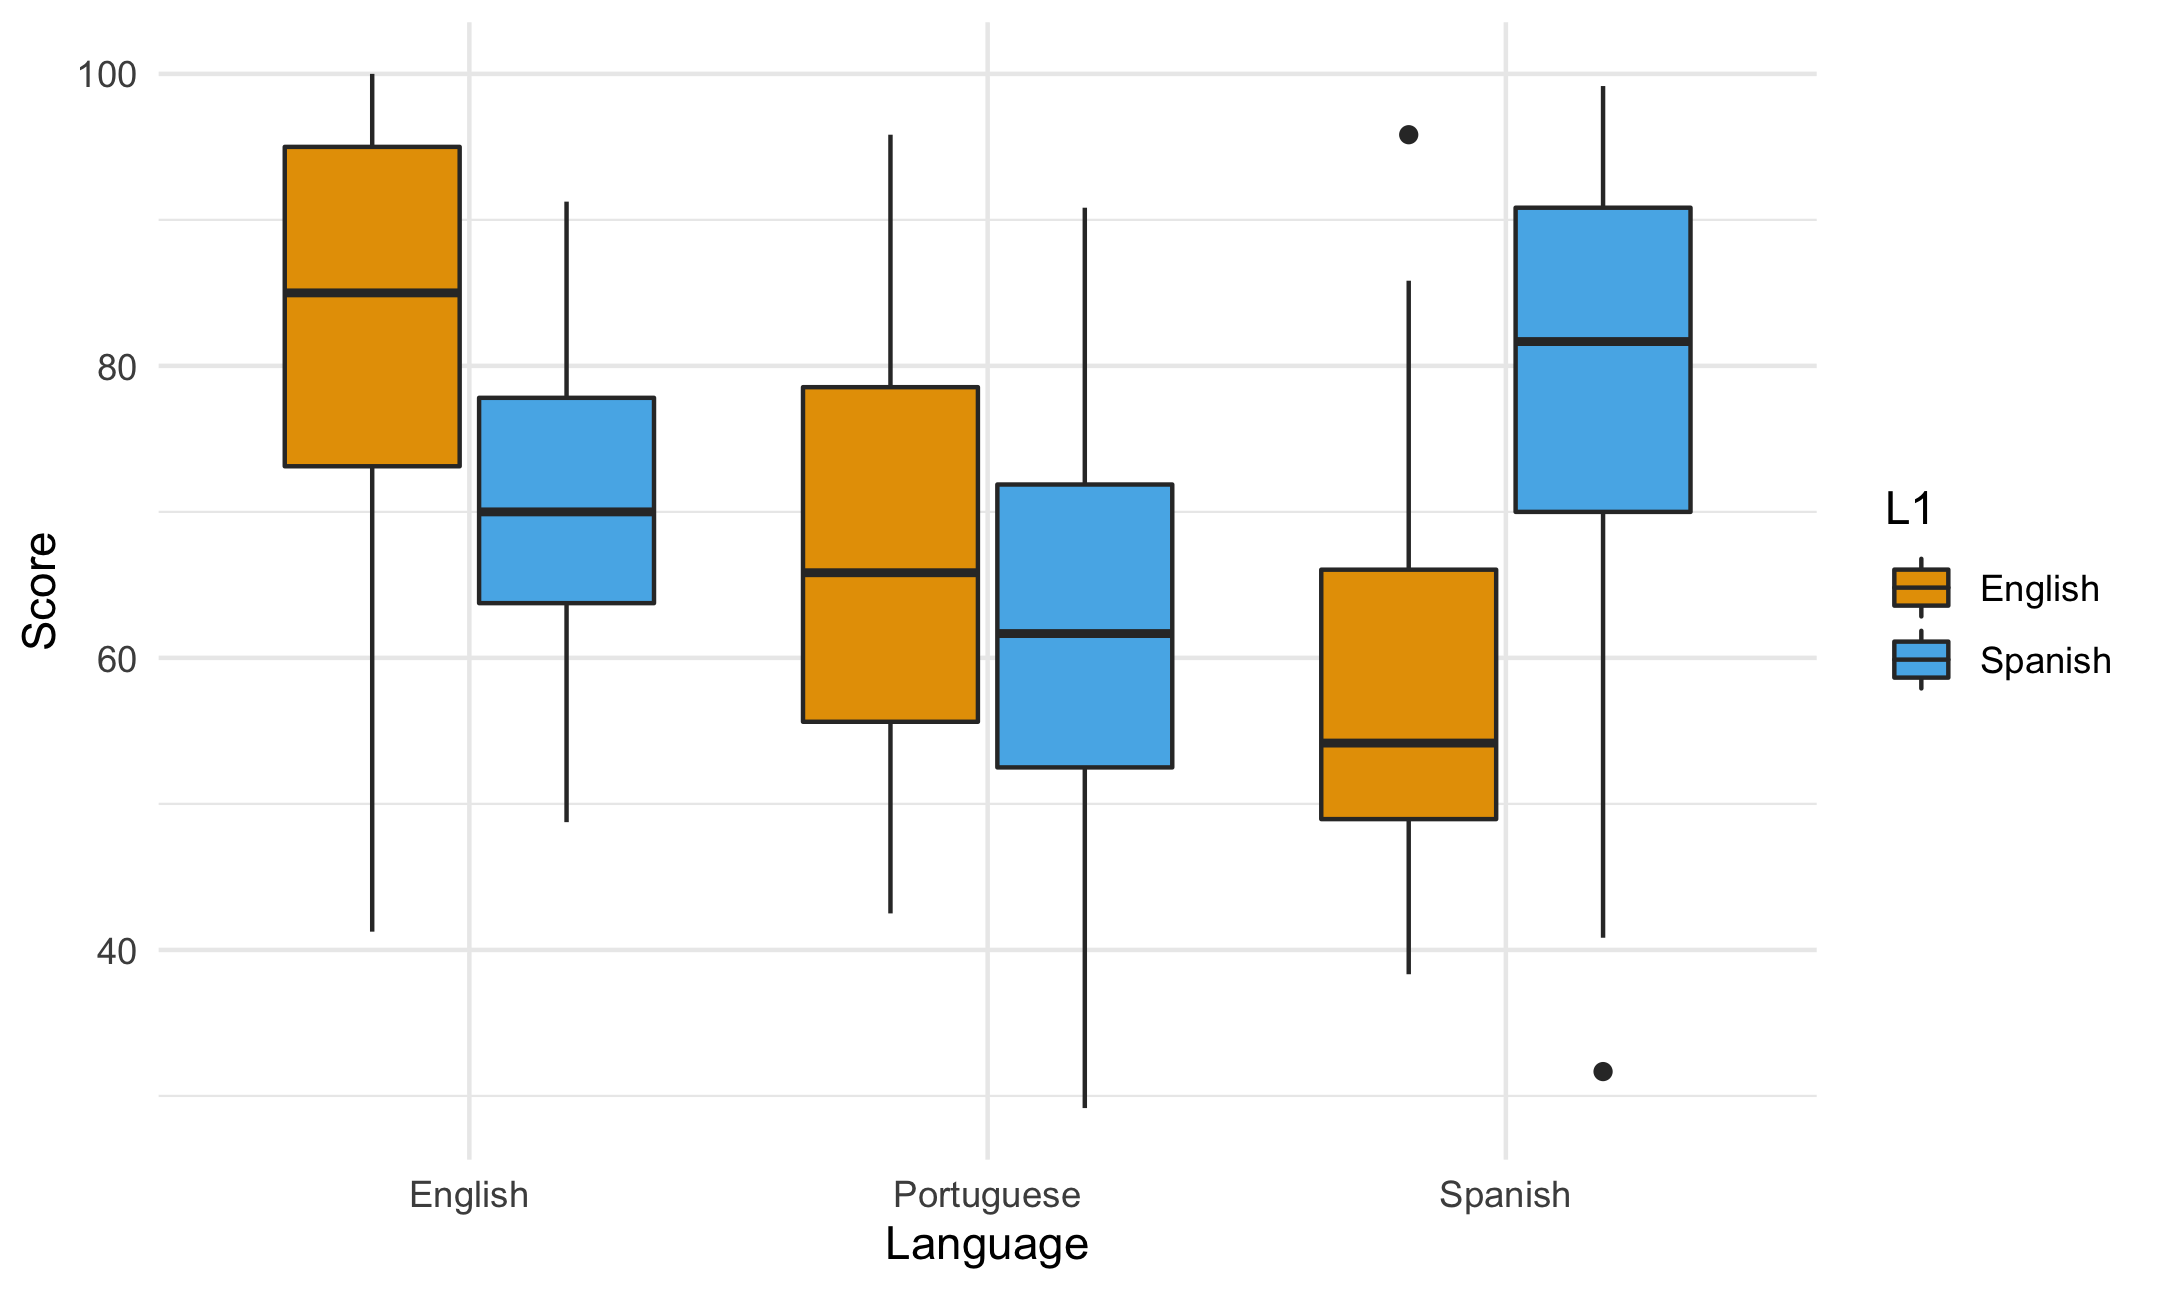
\includegraphics[width=7.19in]{docs/figs/prof_plot} \caption{LexTALE score as a function of Language and Group}\label{fig:prof-desc}
\end{figure}

{[}Insert Figure \ref{fig:prof-desc} about here{]}

\hypertarget{semantic-interpretation-task}{%
\subsubsection{Semantic Interpretation Task}\label{semantic-interpretation-task}}

The semantic interpretation task was designed to measure perception of how adjective-noun order impacts determiner phrase interpretation.
In both Spanish and Portuguese, but not in English, whether an adjective is placed before a noun \emph{el nuevo libro} or after the noun \emph{el libro nuevo} can impact the meaning of the determiner phrase.
For example, \emph{el libro nuevo} refers to a book that has been newly acquired, but is not necessarily brand-new, where \emph{el neuvo libro} does refer to a brand new book.
The task contained 5 target items were tested in each of a pre-nominal and post-nominal condition.
A full list of the stimuli used, along with the correct answers, can be found in the supplementary materials.
Below is an example taken of the Semantic interpretation task in Spanish taken directly from Rothman (2011).

\textbf{Prompt}
``Los maridos honestos se merecen el respeto de sus mujeres.''

\textbf{Answer choices}

a.) \emph{De todos los maridos que hay solo algunos, los que son honestos merecen el respeto de sus esposas.}

b.) Todo marido se merece el respeto de su esposa porque todo marido es, por ser marido, honesto.

\textbf{Prompt}
``Los valientes Incas tenían mucho éxito.''

\textbf{Answer choices}

a.) Entre los incas había los valientes y los no valientes, así que todo inca que era valiente también tenía éxito

b.) \emph{Ser Inca equivale a ser valiente, así que todo Inca tenía éxito.}

\hypertarget{context-based-collocation-task}{%
\subsubsection{Context-based Collocation Task}\label{context-based-collocation-task}}

A second task elicited production of adjectival DPs by way of context.
In the task, participants read a short story and had to fill in a blank at the end of the story with either a pre or post nominal adjective.
Below is an example of the Context-based Collocation Task in Spanish taken directly from Rothman (2011).

\emph{Example}

Mi esposa se llama Magda. Ella es una persona muy amable y cariñosa. Aunque solo tenemos 22 años, hace mucho tiempo que somos amigas. Magda es una vieja amiga \_\_\_\_\_\_\_ (viejo).

`My best friend is named Magda. She is a very nice and affectionate person. Even though we are only 22-years-old, we have been friends for a long time. Magda is an old friend.''

\hypertarget{procedure}{%
\subsection{Procedure}\label{procedure}}

Participants completed all tasks in a single experimental session in the in-browser platform Gorilla.sc (Anwyl-Irvine, Massonnié, Flitton, Kirkham, \& Evershed, 2018).
The session began with a brief history questionnaire, followed by the LexTALE proficiency tests and ended with the two experimental tasks.
The LexTALE test languages were randomized, so any combination of Spanish, English and Portuguese was possible.
The experiments paused briefly between tasks.
All data collection took place asynchronously online on the participant's computer.

\hypertarget{statistical-analysis}{%
\subsection{Statistical analysis}\label{statistical-analysis}}

A replication of the analysis of the original study was carried out.
In the original study, two multilevel two-way ANOVAs for each of the tasks (the Semantic interpretation and context-based collocation tasks) were done.
In each model, the number of correct responses was analyzed as a function of item type (preposed or postposed), group (L1 Spanish, L1 English) and their interaction, with participant included as a random intercept.
Main effects and interactions were assessed using nested model comparisons and model assumptions were verified via visual inspections of Q-Q and residuals vs.~fitted plots.
Post-hoc tests of equivalence were also run when there was not a main effect of a categorical predictor.
In all cases, alpha was set to .05.
In the test of equivalence, the equivalence bounds were +/- Cohen's d = .4.

\hypertarget{results}{%
\section{Results}\label{results}}

Figure \ref{fig:cmc-desc} shows the average correct responses (out of 5) for the Context-based collocation task by all 4 groups, while figure \ref{fig:sem-desc} shows the same information for the Context-based collocation task by all 4 groups.
The means and standard deviations for each case are present just above each bar.
Overall, the participants were more often correct in the postposed condition in both tasks.

{[}Insert Figure \ref{fig:cmc-desc} about here{]}

{[}Insert Figure \ref{fig:sem-desc} here{]}

\begin{figure}
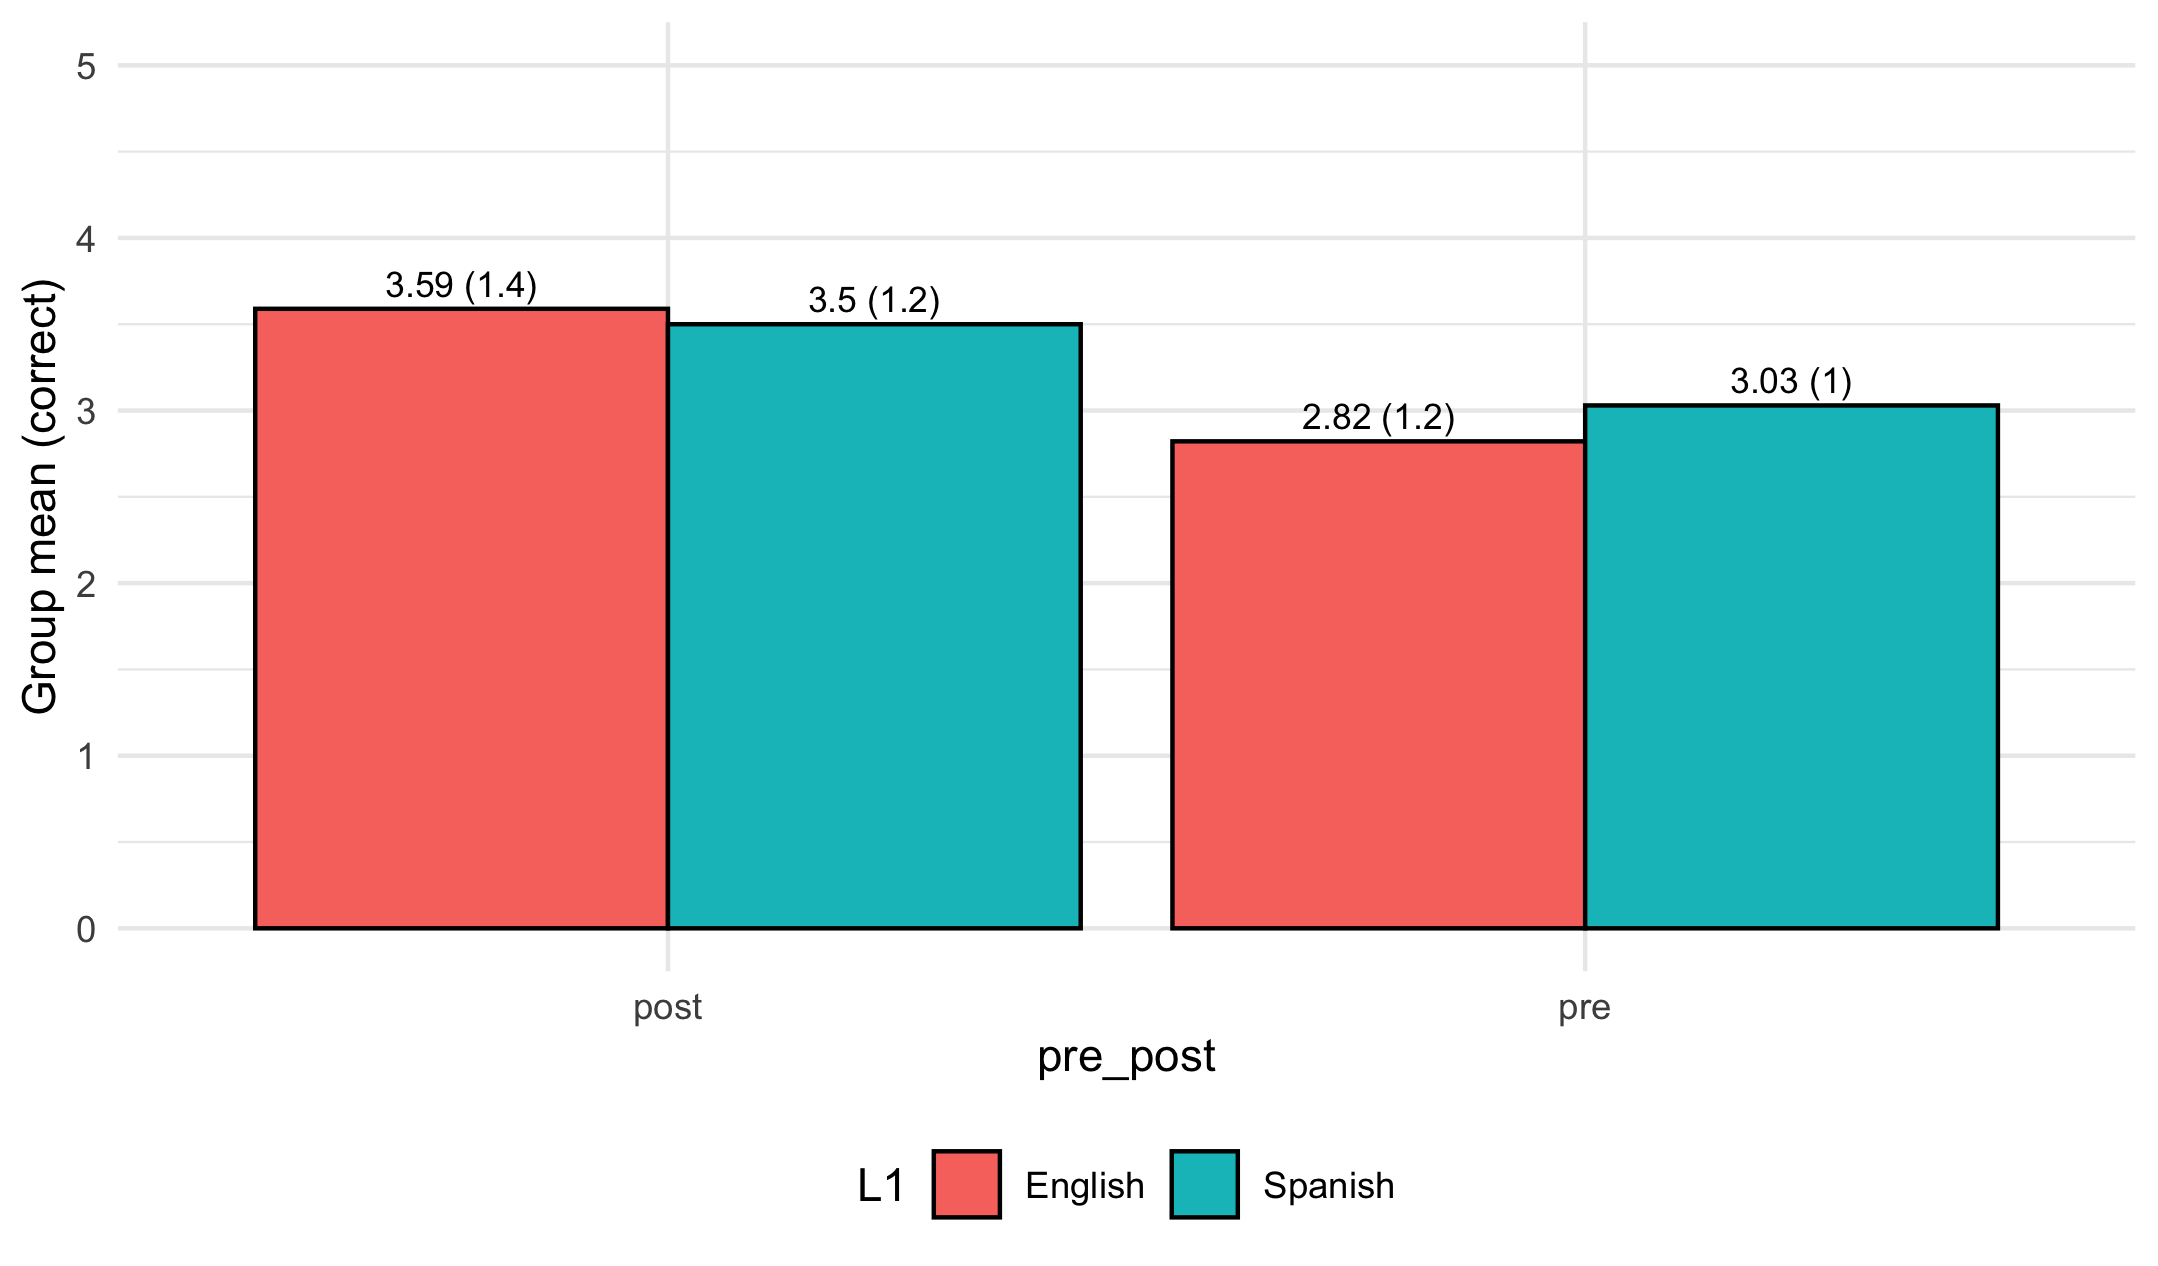
\includegraphics[width=7.19in]{docs/figs/cbc_desc} \caption{Average Number of correct answers in the Context-based Collocation Task}\label{fig:cmc-desc}
\end{figure}

\begin{figure}
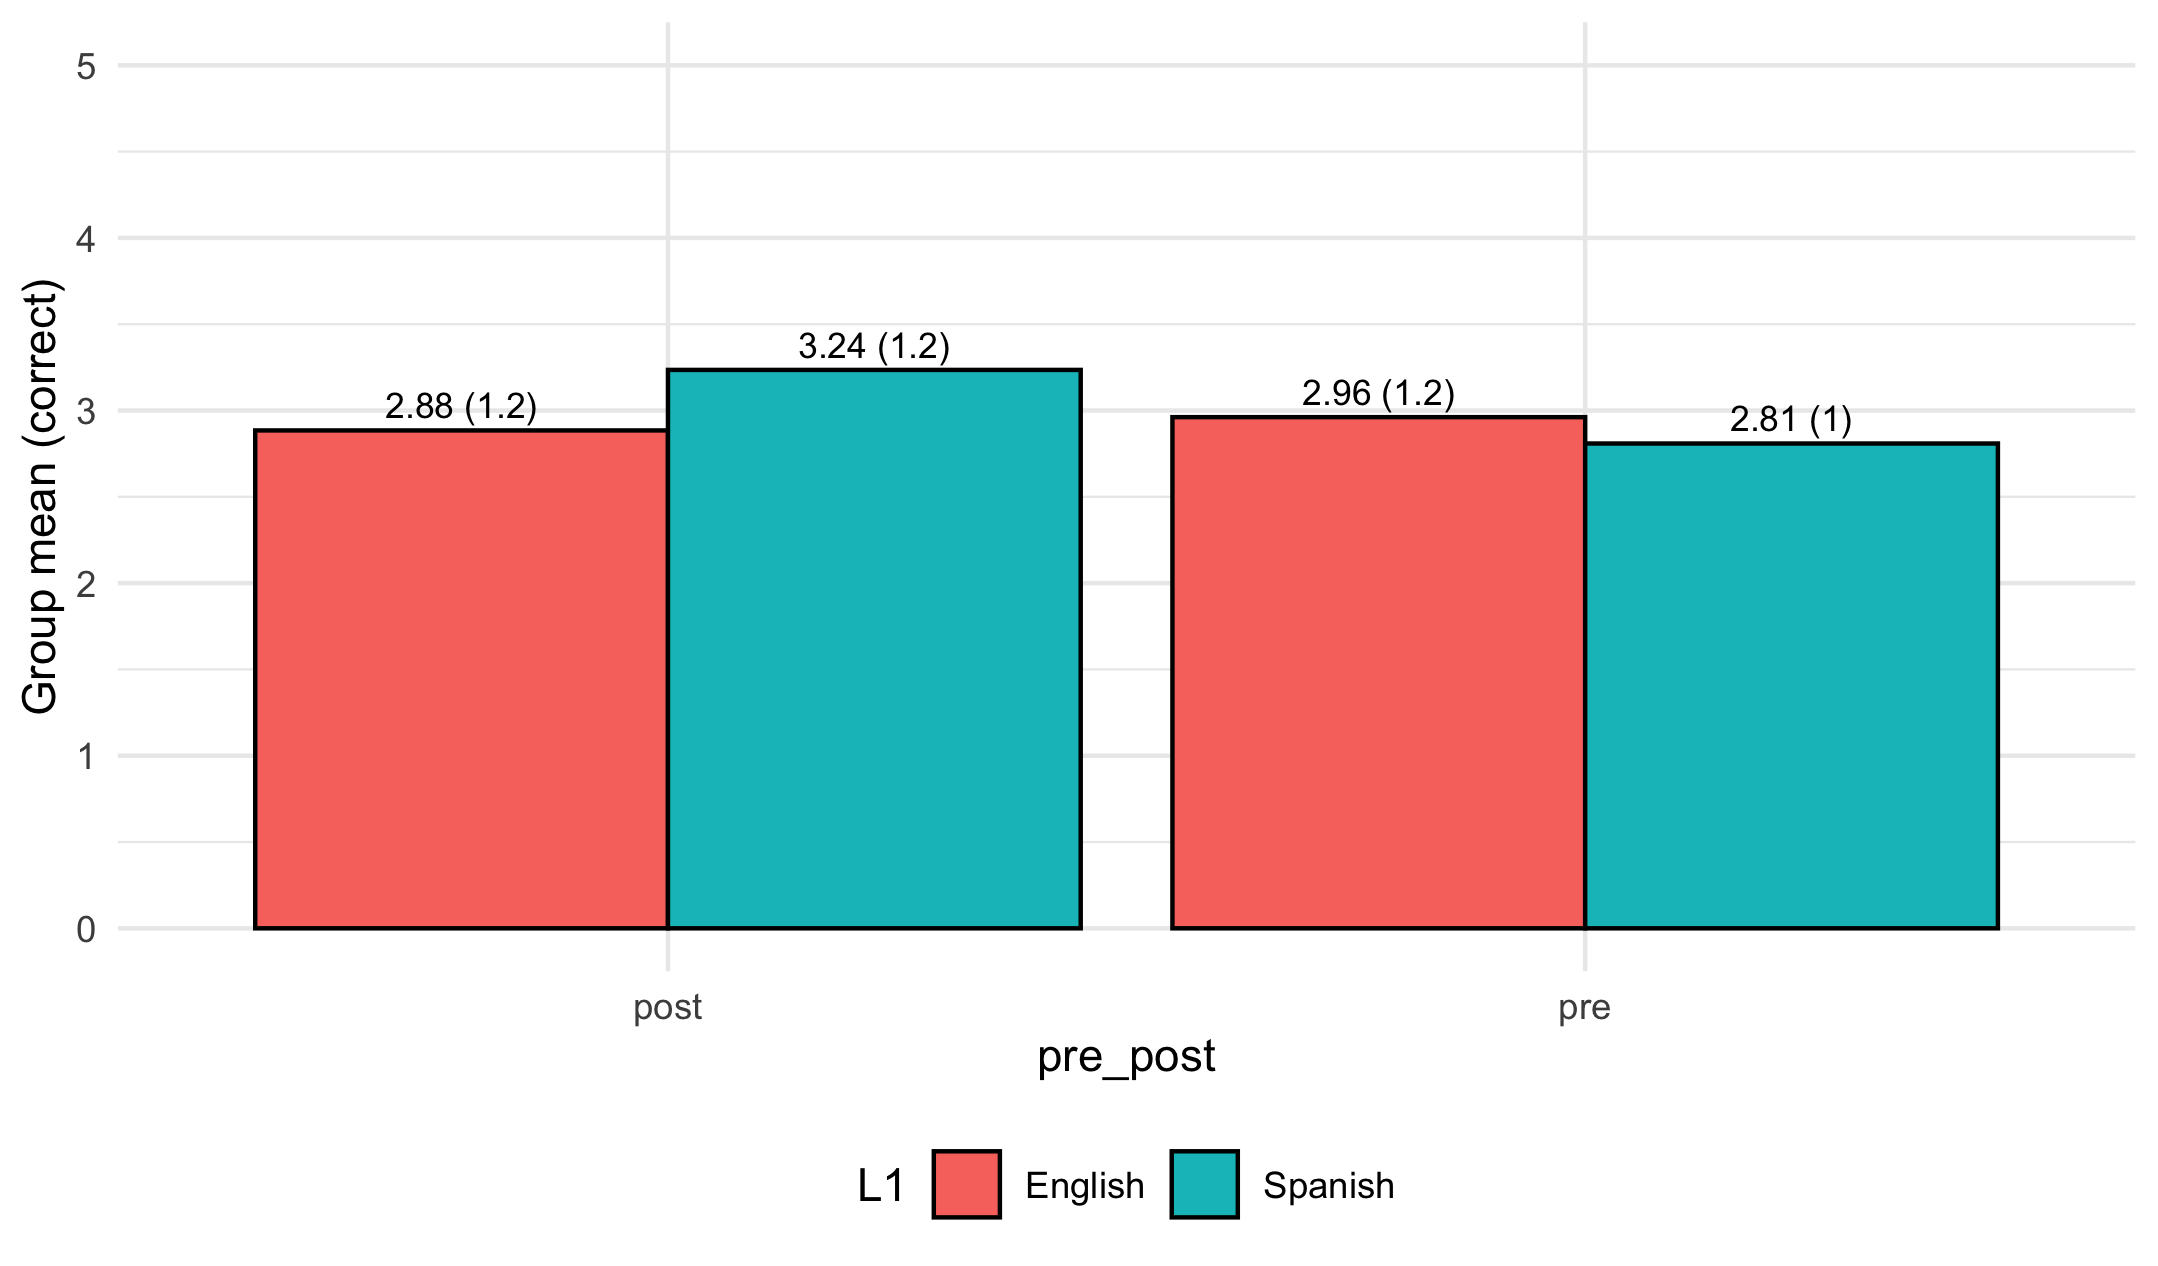
\includegraphics[width=7.19in]{docs/figs/semantic_desc} \caption{Average Number of correct answers in the Semantic Interpretation Task}\label{fig:sem-desc}
\end{figure}

\hypertarget{replication-of-the-original-analysis}{%
\subsubsection{Replication of the original analysis}\label{replication-of-the-original-analysis}}

There was no main effect for group in the ANOVA for the collocation task, F(1, 213) = 0.47, p = 0.50.
There was, however, a main effect for position (pre vs.~post), F(1, 213) = 36.06, p \textgreater{} .05.
There was not a group by position interaction, F(1, 213) = 1.37, p \textgreater{} .05.
In the interpretation task, there was also no main effect for group, F(1, 209) = 0.22, p = 0.64.
Like the collocation task, there was a main effect for position (pre vs.~post), F(1, 209) = 8.41, p \textgreater{} .05.
There was also a group by position interaction, F(1, 209) = 6.72, p \textgreater{} .05.

\hypertarget{test-of-equivalence}{%
\subsubsection{Test of Equivalence}\label{test-of-equivalence}}

In addition to each test of equivalence, a Welch's Two Sample t-test was carried out to determine whether, while also potentially being practically equivalent, a comparison would also be statistically different (see e.g. Lakens et al., 2018).
Each test was run between groups (L1 English and L1 Spanish) for either preposed or postposed adjectives in both the semantic interpretation task and collocation task.

\hypertarget{postposed-collocation}{%
\subsection{Postposed collocation}\label{postposed-collocation}}

The equivalence test was significant in the postposed collocation task, t(207) = -2.65, p = 0.00.
The equivalence bounds were d = +/- .4 or +/- 0.51 in raw units (answers correct).
The observed effect was a mean difference of 0.05 (90\% CI -0.24 - 0.34) in standardized units or 0.04 (90\% CI -0.19 - 0.26) in raw units.
The t-test was not significant, t(207) = 0.28, p = 0.78.
Given these results, we can conclude that the groups were not different from 0 and statistically practically equivalent in their number of correct answers in the postposed condition in the collocation task.

\hypertarget{preposed-collocation-task}{%
\subsection{Preposed collocation task}\label{preposed-collocation-task}}

In the preposed condition on the collocation task, the test of equivalence was significant for the upper bound \(\Delta\)U, t(194.23) = -4.28, p = 0, but not at the lower bound, \(\Delta\)L, t(194.23) = 1.54, p = 0.06.
The equivalence bounds were d = +/- .4 or +/- 0.45 in raw units (answers correct).
The observed effect was a mean difference of -0.21 (90\% CI -0.47 - 0.04) in standardized units or -0.19 (90\% CI -0.41 - 0.04) in raw units.
The t-test was also not significant, t(194) = -1.37, p = 0.17.
Taken together, these results suggest that the effect is not different from zero and also not practically equivalent within a small effect size.

\hypertarget{postposed-semantic-interpretation-task}{%
\subsection{Postposed Semantic interpretation task}\label{postposed-semantic-interpretation-task}}

The equivalence test was significant in the postposed semantic interpretation task, t(199) = -4.12, p = 0.05.
The equivalence bounds were d = +/- .4 or +/- 0.48 in raw units (answers correct).
The observed effect was a mean difference of -0.20 (90\% CI -0.48 - 0.07) in standardized units or -0.17 (90\% CI -0.40 - 0.06) in raw units.
The t-test was not significant, t(198.98) = 0.28, p = 0.78.
Given these results, we can conclude that the groups were not different from 0 and statistically practically equivalent in their number of correct answers in the postposed condition in the collocation task.

\hypertarget{preposed-semantic-interpretation-task}{%
\subsection{Preposed Semantic interpretation task}\label{preposed-semantic-interpretation-task}}

In the preposed condition on the semantic interpretation task, the test of equivalence was not significant for the upper bound \(\Delta\)U, t(194.23) = -4.28, p = 0, but was at the lower bound, \(\Delta\)L, t(194.23) = 1.54, p = 0.06.
The equivalence bounds were d = +/- .4 or +/- 0.45 in raw units (answers correct).
The observed effect was a mean difference of -0.21 (90\% CI -0.47 - 0.04) in standardized units or -0.19 (90\% CI -0.41 - 0.04) in raw units.
The t-test was significant, t(198.71) = 2.10, p = 0.04.
Taken together, these results suggest that the groups were statistically different in their number of correct answers and not practically equivalent within a small effect size.

\hypertarget{discussion-and-conclusion}{%
\section{Discussion and conclusion}\label{discussion-and-conclusion}}

\hypertarget{summary-of-results}{%
\subsection{Summary of results}\label{summary-of-results}}

\begin{longtable}[]{@{}lrr@{}}
\caption{\label{tab:summaryanovas}Summary of the Analyses of Variance in both tasks}\tabularnewline
\toprule
\endhead
Task & Collocation Task & Semantic Interpretation Task \\
Group & no & no \\
ANOVA\_position & yes & yes \\
ANOVA\_interaction & no & yes \\
Replication & Partial & Partial \\
\bottomrule
\end{longtable}

{[}Insert Table \ref{tab:summaryanovas} about here{]}

Table \ref{tab:summaryanovas} summarizes the results of the replication of the original analyses.
Overall, the results of the two ANOVAs point to a partial replication.
The original study reported no main effects or interactions.
The present study found no main effects for group, but did for position in both tasks and an interaction for the Semantic Interpretation task.
Table \ref{tab:summaryttests} details results of the tests of equivalence.
The four total tests compared the number of correct answers out of five for both tasks in preposed and postposed positions.
The results showed that two of the four comparisons were practically equivalent, while they other two were not, when the equivalence bounds were d = +/- .4.

{[}Insert Table \ref{tab:summaryttests} about here{]}

\begin{longtable}[]{@{}rrrr@{}}
\caption{\label{tab:summaryttests}Summary of the results from the tests of equivalence and t-tests}\tabularnewline
\toprule
Position & Task & TOST & t\_test \\
\midrule
\endfirsthead
\toprule
Position & Task & TOST & t\_test \\
\midrule
\endhead
pre & Collocation Task & no & no \\
post & Collocation Task & yes & no \\
pre & Semantic Interpretation Task & no & no \\
post & Semantic Interpretation Task & yes & no \\
\bottomrule
\end{longtable}

\hypertarget{implications-for-statistical-tools-used-in-l3-acquisition}{%
\section{Implications for statistical tools used in L3 acquisition}\label{implications-for-statistical-tools-used-in-l3-acquisition}}

While the present results reinforce the idea that typological similarity plays a role in third language acquisition, they also suggest that careful use of statistical tools and tempered conclusions can improve models moving forward.
In the present study, like in Rothman (2011), there was no main effect of group.
In many studies, this result has been taken as evidence of (practically) equivalent performance between groups.
However, the present study only found that this was the case in two of the four possible cases.
Thus, the interpretation of results in a frequentist framework should not simply be binary, in which results are interpreted as either significant (different) or not significant (the same).
Rather, null effects should be considered as a inconclusive, since they, in and of themselves, do not provide evidence for equivalent performance between groups.
Lago (2021) pointed out this issue, stating that absence of evidence does not constitute evidence of absence (Altman \& Bland, 1995).

One method to determine whether an experiment with null results can also claim practical equivalence is doing a post-hoc test of equivalence.
In so doing, the researcher must determine equivalence bounds based on theory.
Arguably, this method is a joining to (linguistic) theory and the statistical tools linguists use to draw conclusions, since it is a departure from the more or less arbitrary thresholds commonly used in research in the social sciences, such as the significance threshold of .05 or a power level of .8.
Interestingly, if we SESOI was simply d = +/- .5, all four tests of equivalence would have been significant.
On a raw scale, this would be setting equivalence to +/- .6 answers correct (12 percent) as opposed to +/- .48 answers correct (9.6 percent).
Given that these bounds were chosen as a bench mark, it's unclear whether either was truly a better choice for practical equivalence.
Overall, the nature of evidence taken as support for wholesale transfer should be re-considered, with specific interest in determining the SESOI on a given task.

One potential way to determine the smallest effect size of interest and conduct power analyses.
The present study considered the d = +/- .4 as the SESOI based on a recent meta-analysis of effect sizes in L2 research (@ Plonsky \& Oswald, 2014).
Other L2 studies could consider this as a general benchmark, but also can and should consider other effect sizes.
Figure \ref{fig:pc} shows the needed participants per group to detect practical equivalence at a power level of .8 (alpha = .05) according do the smallest effect size of interest ranging from d = +/-.1 to +/- 1.
The smallest effect size of interest was used as the equivalence bounds, meaning that any effect less than the SESOI was considered practically equivalent.
It is clear from the figure that evidence for the null hypothesis requires a rather large sample in the event that a very small effect is considered meaningful.
For example, if the sesoi is d = +/- .1, then 1713 participants are needed per group to achieve a power level of .8.
On the other hand, if only a large effect is considered meaningful, such as d = +/- 1, then only 17 participants are needed per group.

Another way of understanding the consequences of over-extrapolation of small samples is to better quantify the uncertainty related to the statistical power of a given hypothesis test.
That is, if a study includes a small sample and finds a null effect, practical equivalence can only reliably be found when the equivalence bounds are wide.
For example, the statistical power of detecting practical equivalence when each group has 17 participants, the equivalence bounds are d = +/- .4, and alpha = .05 is 0.
This results suggests that it was practically impossible for the original study to draw a practically equivalent sample.
Rather, a sample of 17 per group (the biggest group from the original study) when alpha is .05 only has a power level of .8 when the equivalence bounds are d = +/- 1.
To make another example that is more practical to the present design, given our pooled standard deviation of 1.2, this difference would equal a mean difference between groups of 1.2 correct answers or 24\%.
The higher sample, however, can conclude with a probability of .8 that practical equivalence between groups is within .48 correct answers, or 9.6\%.
In most cases, it seems plausible that a difference of 24\% is considered to be a meaningful.
Take, for example, grades in the University system of the United States, where such a difference amounts to more than two letter grades in difference.

{[}Insert Figure \ref{fig:pc} about here{]}

\begin{figure}
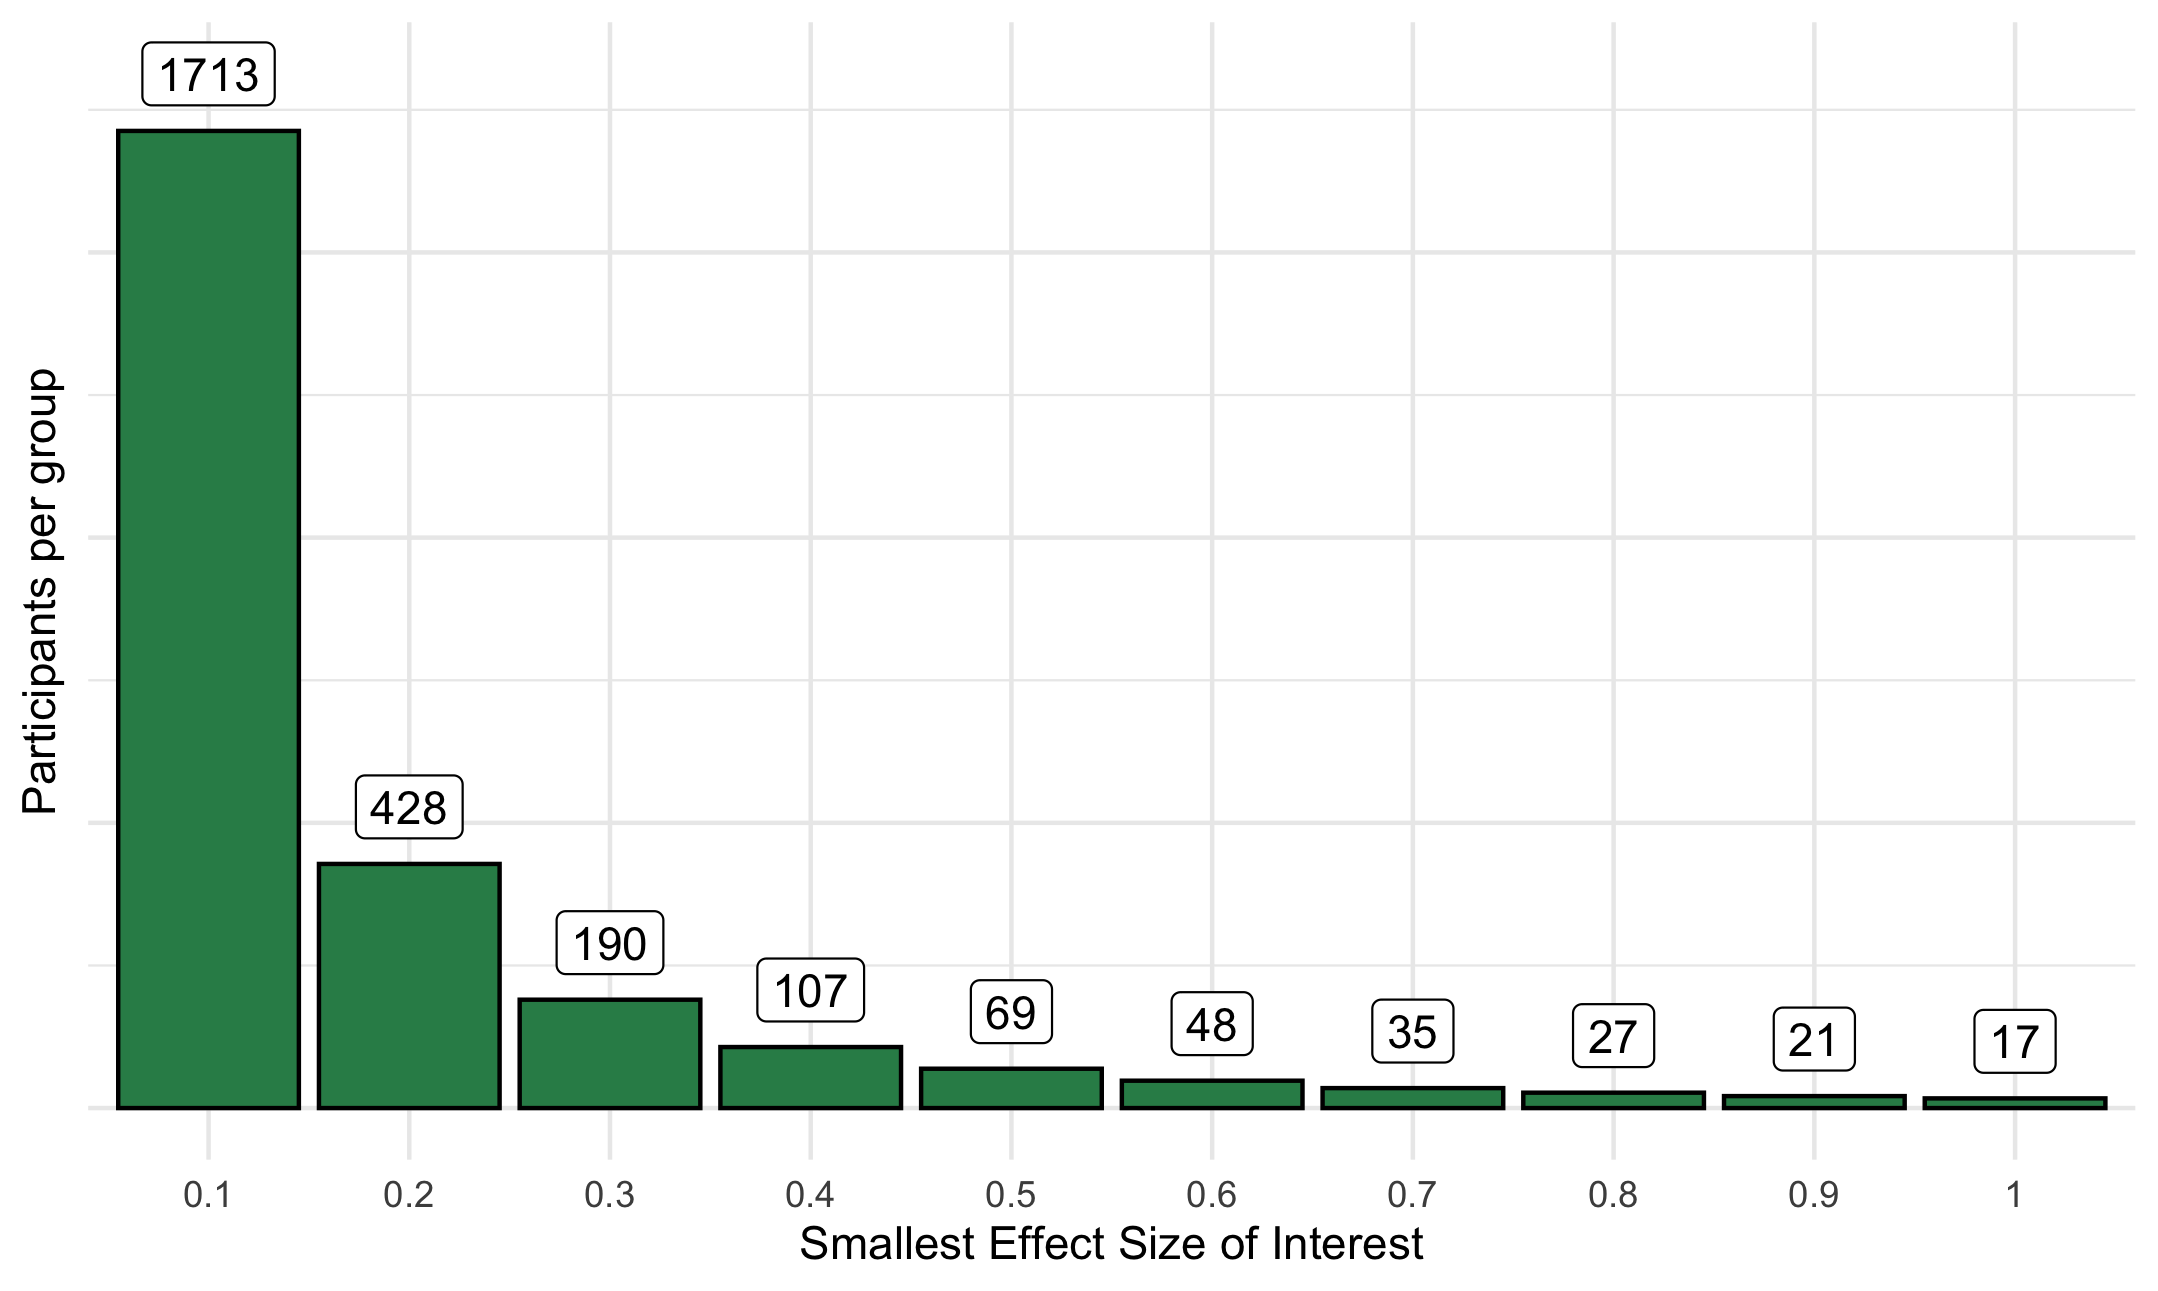
\includegraphics[width=7.19in]{docs/figs/pc} \caption{Number of participants needed according to the smallest effect size of interest}\label{fig:pc}
\end{figure}

\hypertarget{implcations-for-l3-theory}{%
\section{Implcations for L3 theory}\label{implcations-for-l3-theory}}

This result reinforces the view that the typological similarity between the L3 and learned languages plays an important role in L3 acquisition.
However, these results on their own do not necessarily provide evidence of wholesale transfer, since only one linguistic structure was tested (see e.g. Marsden, 2021).
As a result, the present results are best explained by typology-based models, the TPM, the LPM, the CEM and the Scalpel Model, given that Spanish appears to have influenced the participants' judgments in their L3 Portuguese whether or not it was their first or second language.

It is important to note that the evidence for wholesale transfer has primarily come from studies with one structure that also use null results are evidence for equivalence.
As a result, it cannot be concluded from this replication alone whether wholesale transfer occurs, nor whether both groups are equally impacted by their Spanish, since the only two of four possible comparisons were practically equivalent.
Here, I have suggested the use of more sensitive statistical tools, such as tests of equivalence, with a given effect size in mind prior to data collection.

\newpage

\hypertarget{references}{%
\section{References}\label{references}}

\begingroup
\setlength{\parindent}{-0.5in}
\setlength{\leftskip}{0.5in}

\hypertarget{refs}{}
\begin{CSLReferences}{1}{0}
\leavevmode\vadjust pre{\hypertarget{ref-altman1995statistics}{}}%
Altman, D. G., \& Bland, J. M. (1995). Statistics notes: Absence of evidence is not evidence of absence. \emph{Bmj}, \emph{311}(7003), 485.

\leavevmode\vadjust pre{\hypertarget{ref-anwyl2018gorillas}{}}%
Anwyl-Irvine, A., Massonnié, J., Flitton, A., Kirkham, N., \& Evershed, J. (2018). Gorillas in our midst: Gorilla. sc. \emph{Behavior Research Methods}.

\leavevmode\vadjust pre{\hypertarget{ref-bardel2007role}{}}%
Bardel, C., \& Falk, Y. (2007). The role of the second language in third language acquisition: The case of germanic syntax. \emph{Second Language Research}, \emph{23}(4), 459--484.

\leavevmode\vadjust pre{\hypertarget{ref-bardel2012l2}{}}%
Bardel, C., \& Falk, Y. (2012). The L2 status factor and the declarative/procedural distinction. \emph{Third Language Acquisition in Adulthood}, \emph{46}, 61--78.

\leavevmode\vadjust pre{\hypertarget{ref-flynn2004cumulative}{}}%
Flynn, S., Foley, C., \& Vinnitskaya, I. (2004). The cumulative-enhancement model for language acquisition: Comparing adults' and children's patterns of development in first, second and third language acquisition of relative clauses. \emph{International Journal of Multilingualism}, \emph{1}(1), 3--16.

\leavevmode\vadjust pre{\hypertarget{ref-grosjean1989neurolinguists}{}}%
Grosjean, F. (1989). Neurolinguists, beware! The bilingual is not two monolinguals in one person. \emph{Brain and Language}, \emph{36}(1), 3--15.

\leavevmode\vadjust pre{\hypertarget{ref-hermas2010language}{}}%
Hermas, A. (2010). Language acquisition as computational resetting: Verb movement in L3 initial state. \emph{International Journal of Multilingualism}, \emph{7}(4), 343--362.

\leavevmode\vadjust pre{\hypertarget{ref-hermas2014multilingual}{}}%
Hermas, A. (2014). Multilingual transfer: L1 morphosyntax in L3 english. \emph{International Journal of Language Studies}, \emph{8}(2), 1--24.

\leavevmode\vadjust pre{\hypertarget{ref-izura2014lextale}{}}%
Izura, C., Cuetos, F., \& Brysbaert, M. (2014). Lextale-esp: A test to rapidly and efficiently assess the spanish vocabulary size. \emph{Psicol{ó}gica}, \emph{35}(1), 49--66.

\leavevmode\vadjust pre{\hypertarget{ref-jin2009third}{}}%
Jin, F. (2009). Third language acquisition of norwegian objects: Interlanguage transfer or L1 influence. \emph{Third Language Acquisition and Universal Grammar}, 144--161.

\leavevmode\vadjust pre{\hypertarget{ref-lago2021some}{}}%
Lago, S. (2021). Some challenges of relating wholesale transfer approaches to L3 linguistic behavior. \emph{Linguistic Approaches to Bilingualism}, \emph{11}(1), 75--78.

\leavevmode\vadjust pre{\hypertarget{ref-lakens2018equivalence}{}}%
Lakens, D., Scheel, A. M., \& Isager, P. M. (2018). Equivalence testing for psychological research: A tutorial. \emph{Advances in Methods and Practices in Psychological Science}, \emph{1}(2), 259--269.

\leavevmode\vadjust pre{\hypertarget{ref-lemhofer2012introducing}{}}%
Lemhöfer, K., \& Broersma, M. (2012). Introducing LexTALE: A quick and valid lexical test for advanced learners of english. \emph{Behavior Research Methods}, \emph{44}, 325--343.

\leavevmode\vadjust pre{\hypertarget{ref-marsden2021there}{}}%
Marsden, H. (2021). When there's no mirror image, and other L3 research design challenges. \emph{Linguistic Approaches to Bilingualism}, \emph{11}(1), 79--83.

\leavevmode\vadjust pre{\hypertarget{ref-plonsky2014big}{}}%
Plonsky, L., \& Oswald, F. L. (2014). How big is {``big''}? Interpreting effect sizes in L2 research. \emph{Language Learning}, \emph{64}(4), 878--912.

\leavevmode\vadjust pre{\hypertarget{ref-puig2020systematic}{}}%
Puig-Mayenco, E., González Alonso, J., \& Rothman, J. (2020). A systematic review of transfer studies in third language acquisition. \emph{Second Language Research}, \emph{36}(1), 31--64.

\leavevmode\vadjust pre{\hypertarget{ref-puig2020low}{}}%
Puig-Mayenco, E., \& Rothman, J. (2020). Low proficiency does not mean ab initio: A methodological footnote for linguistic transfer studies. \emph{Language Acquisition}, \emph{27}(2), 217--226.

\leavevmode\vadjust pre{\hypertarget{ref-rothman2011l3}{}}%
Rothman, J. (2011). L3 syntactic transfer selectivity and typological determinacy: The typological primacy model. \emph{Second Language Research}, \emph{27}(1), 107--127.

\leavevmode\vadjust pre{\hypertarget{ref-rothman2015linguistic}{}}%
Rothman, J. (2015). Linguistic and cognitive motivations for the typological primacy model (TPM) of third language (L3) transfer: Timing of acquisition and proficiency considered. \emph{Bilingualism: Language and Cognition}, \emph{18}(2), 179--190.

\leavevmode\vadjust pre{\hypertarget{ref-schwartz1996l2}{}}%
Schwartz, B. D., \& Sprouse, R. A. (1996). L2 cognitive states and the full transfer/full access model. \emph{Second Language Research}, \emph{12}(1), 40--72.

\leavevmode\vadjust pre{\hypertarget{ref-schwartz2021full}{}}%
Schwartz, B. D., \& Sprouse, R. A. (2021). The full transfer/full access model and L3 cognitive states. \emph{Linguistic Approaches to Bilingualism}, \emph{11}(1), 1--29.

\leavevmode\vadjust pre{\hypertarget{ref-slabakova2017scalpel}{}}%
Slabakova, R. (2017). The scalpel model of third language acquisition. \emph{International Journal of Bilingualism}, \emph{21}(6), 651--665.

\leavevmode\vadjust pre{\hypertarget{ref-westergaard2017crosslinguistic}{}}%
Westergaard, M., Mitrofanova, N., Mykhaylyk, R., \& Rodina, Y. (2017). Crosslinguistic influence in the acquisition of a third language: The linguistic proximity model. \emph{International Journal of Bilingualism}, \emph{21}(6), 666--682.

\leavevmode\vadjust pre{\hypertarget{ref-zhou2022lextpt}{}}%
Zhou, C., \& Li, X. (2022). LextPT: A reliable and efficient vocabulary size test for L2 portuguese proficiency. \emph{Behavior Research Methods}, \emph{54}(6), 2625--2639.

\end{CSLReferences}

\endgroup


\end{document}
